\chapter{Implementation of methods}
\label{cha:implementation_methods}

As many pattern recognition techniques were originally not designed to cope with large amounts of irrelevant features, combining them with FS techniques has become a necessity in many applications (Guyon and Elisseeff, 2003; Liu and Motoda, 1998; Liu and Yu, 2005). The objectives of feature selection are manifold, the most important ones being: (a) to avoid overfitting and improve model performance, i.e. prediction performance in the case of supervised classification and better cluster detection in the case of clustering, (b) to provide faster and more cost-effective models and (c) to gain a deeper insight into the underlying processes that generated the data. However, the advantages of feature selection techniques come at a certain price, as the search for a subset of relevant features introduces an additional layer of complexity in the modelling task. Instead of just optimizing the parameters of the model for the full feature subset, we now need to find the optimal model parameters for the optimal feature subset, as there is no guarantee that the optimal parameters for the full feature set are equally optimal for the optimal feature subset (Daelemans et al., 2003). As a result, the search in the model hypothesis space is augmented by another dimension: the one of finding the optimal subset of relevant features. Feature selection techniques differ from each other in the way they incorporate this search in the added space of feature subsets in the model selection.

In the context of classification, feature selection techniques can be organized into three categories, depending on how they combine the feature selection search with the construction of the classification model: filter methods, wrapper methods and embedded methods. Table 1 provides a common taxonomy of feature selection methods, showing for each technique the most prominent advantages and disadvantages, as well as some examples of the most influential techniques.


----------------------------------------------------------



\section{Feature Extraction methods} % (fold)
\label{sec:feature_selection}

\subsection{PCA - Principal Component Analysis} % (fold)
\label{sec:pca}

\begin{lstlisting}[language=Python]
# Calculate the variance explained by principle components
print("Variance_of_each_component:", pca.explained_variance_ratio_)
print("Total_Variance:Explained:", 
        round(sum(list(pca.explained_variance_ratio_))*100, 2))
\end{lstlisting}



\begin{figure}[h]
    \centering
    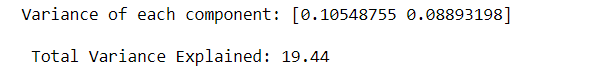
\includegraphics[width=0.8\textwidth,height=0.06\textheight]{Chapters/Figures/pca_2_comp_variance.png}
    \caption{Variance of the best 2 components and their sum}
    \label{fig:total_variance}
\end{figure}


\begin{figure}[h]
    \centering
    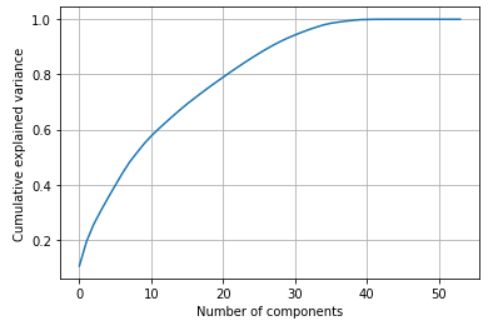
\includegraphics[width=0.75\textwidth,height=0.3\textheight]{Chapters/Figures/number_of_components.png}
    \caption{Cumulative Explained Variance\\ as a function of the Number of Components}
    \label{fig:variance_graph}
\end{figure}




\subsection{SOM - Self Organizing Maps} % (fold)
\label{sec:som}

\subsection{LDA - Linear Driscriminant Analysis} % (fold)
\label{sec:lda}

\section{Feature Selection methods} % (fold)
\label{sec:feature_extraction}


\subsection{Univariate Filtering} % (fold)
\label{sec:inserting_tables}

\subsubsection{Chi-Square test} % (fold)
\label{sec:inserting_tables}

\subsubsection{ANOVA F-test} % (fold)
\label{sec:inserting_tables}

\subsection{Multivariate Filtering} % (fold)
\label{sec:inserting_tables}

\subsubsection{CFS – Correlation Based Feature Selection} % (fold)
\label{sec:inserting_tables}

\subsubsection{MRMR – Minimum Redundancy Maximum Relevance} % (fold)
\label{sec:inserting_tables}